  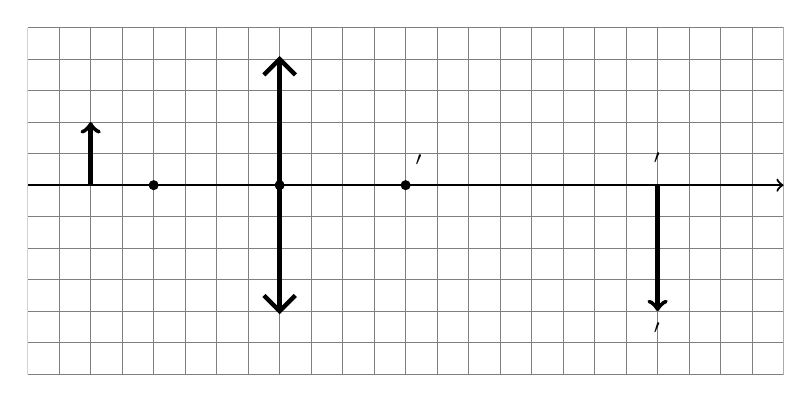
\begin{tikzpicture}[scale=0.8]
    \clip (-4,-3) rectangle (8,2.5) ; %Les dimensions de l'image
    \draw [help lines] (-4,-3) grid [step=0.5] (8,2.5) ; %% Le quadrillage
    \draw [->,thick] (-4,0) -- (8,0) ; %% L'axe optique
    \draw [ultra thick] (0,-2) -- (0,2)  ; %% Le corps du système 
    
    \draw [ultra thick] (-0.25,-1.75) -- (0,-2) -- (0.25,-1.75)
                         (-0.25,1.75) -- (0,2) -- (0.25,1.75) ;                    %La lentille

    \filldraw [black] (0,0) circle (2pt) node [above right] {$\ptO$} ;  %Le centre optique
    \filldraw [black] (2.0,0) circle (2pt) node [above right] {$\ptF'$}; %Le foyer image
    \filldraw [black] (-2.0,0) circle (2pt) node [above left] {$\ptF$} ; %Le foyer objet
    
      \draw [->,ultra thick] (-3,0) node [below] {$\ptA$} -- (-3,1.0) node [above] {$\ptB$} ;   %L'objet
      \draw [->,ultra thick] (6,0) node [above] {$\ptA'$} -- (6,-2.0) node [below] {$\ptB'$} ;     %L'image
      
  \end{tikzpicture}